\RequirePackage[ngerman=ngerman-x-latest]{hyphsubst}
\documentclass[a4paper,12pt,twoside]{article}

\usepackage[ngerman]{babel}
\usepackage{fancyhdr}
\usepackage{graphicx}
\setlength\abovecaptionskip{4pt}
\usepackage[bookmarksopen=true,bookmarksnumbered=true]{hyperref}
\usepackage[utf8]{inputenc}
\usepackage[inner=2.5cm,outer=2cm,top=2.3cm,bottom=2cm,head=0.8cm,headsep=0.8cm,footskip=1cm,asymmetric]{geometry}
\usepackage{setspace}
\usepackage{courier}
\usepackage{array}
\usepackage{amsmath}
\usepackage{amssymb}

\usepackage[babel, german=quotes]{csquotes}

\usepackage[backend=biber,style=apa,citestyle=authoryear-comp, language=autocite, doi=false, isbn=false]{biblatex}
\DeclareLanguageMapping{ngerman}{ngerman-apa}
\addbibresource{master.bib}
\bibliography{master.bib}

\newcommand{\Fb}[1]{\textit{#1}} %Fachbegriff

\usepackage{listings}
\usepackage[dvipsnames]{xcolor}
\lstset{ % 
  language=C++,                % the language of the code 
  frame=single,
  basicstyle=\footnotesize,           % the size of the fonts that are used for the code 
  numbers=left,                   % where to put the line-numbers 
  numberstyle=\tiny\color{gray},  % the style that is used for the line-numbers 
  stepnumber=2,                   % the step between two line-numbers. If it's 1, each line 
                                  % will be numbered 
  numbersep=5pt,                  % how far the line-numbers are from the code 
  backgroundcolor=\color{white},      % choose the background color. You must add \usepackage{color} 
  showspaces=false,               % show spaces adding particular underscores 
  showstringspaces=false,         % underline spaces within strings 
  showtabs=false,                 % show tabs within strings adding particular underscores 
  rulecolor=\color{black},        % if not set, the frame-color may be changed on line-breaks within not-black text 
  tabsize=2,                      % sets default tabsize to 2 spaces 
  captionpos=b,                   % sets the caption-position to bottom 
  breaklines=true,                % sets automatic line breaking 
  breakatwhitespace=false,        % sets if automatic breaks should only happen at whitespace 
  title=\lstname,                   % show the filename of files included with \lstinputlisting; 
                                  % also try caption instead of title 
  keywordstyle=\color{blue},          % keyword style 
  commentstyle=\color{PineGreen},       % comment style 
  stringstyle=\color{Orchid},         % string literal style 
  escapeinside={\%*}{*)},            % if you want to add a comment within your code
  aboveskip=20pt
} 
%\usepackage[german]{babel}

% Nummer des Themas
\newcommand{\No}{$136$}
% Name des Themas
\newcommand{\Theme}{Multi-threaded Query Processing II}
% Name   
\newcommand{\Name}{Ingo Bader}

\onehalfspacing

\nopagebreak

\fancyhead[RE,LO]{\fontsize{9}{9}\selectfont\Theme}
\fancyhead[LE,RO]{\fontsize{9}{9}\selectfont Seite \thepage}
\fancyfoot{}

\begin{document}


% Titelseite
\thispagestyle{empty}
\pagestyle{empty}

\begin{center}
\begin{huge}
\vspace*{3cm}
%      \vspace*{\fill}
    \begin{tabular}{m{1.2cm}@{\ \ }m{9cm}}
      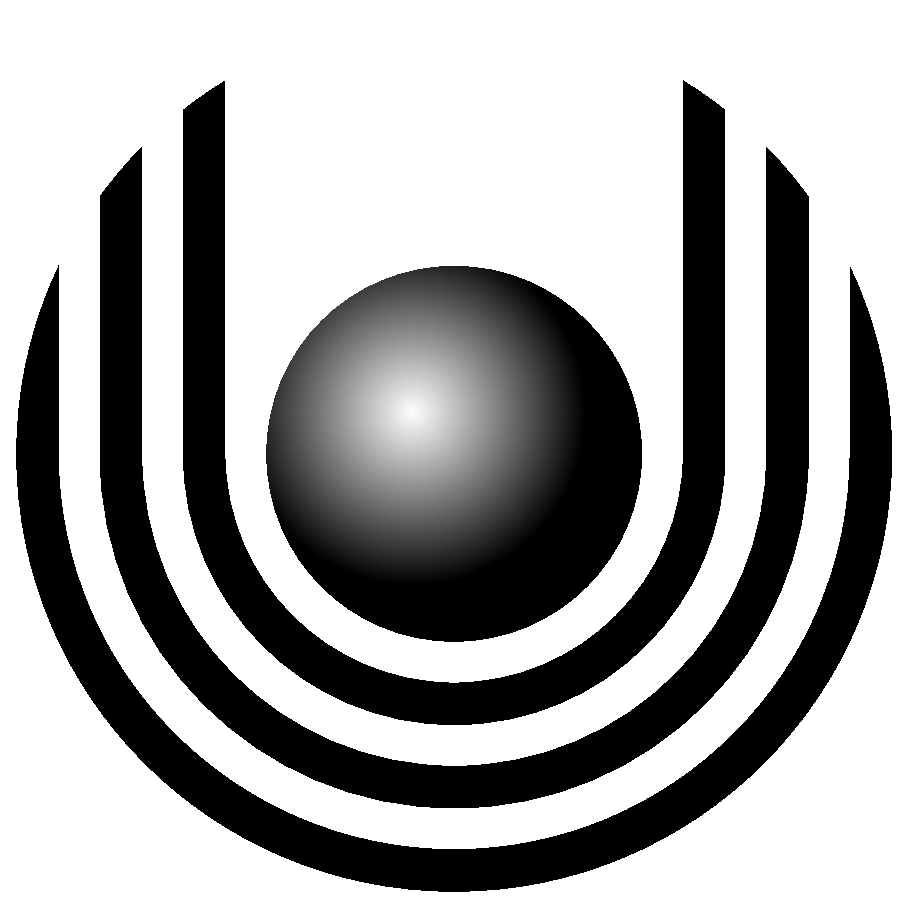
\includegraphics[width=1.2cm]{logo.eps} & {FernUniversität in Hagen}
    \end{tabular}
    \\
    \vspace*{3cm}
   Masterarbeit \\
   Sommersemester 2019 \\[2em]
   \glqq{}Multi-threaded Query Processing II\grqq{} \\[2cm]
\end{huge}
\begin{large}
   Thema \No\\[1em]
   \Theme\\[3cm]
   \Name
\end{large}
\end{center}

\clearpage
\tableofcontents
\clearpage
\raggedbottom
\thispagestyle{fancy}
\pagestyle{fancy}
\setcounter{page}{1}

% Inhalt
\section{Einleitung} (2-3 S)n

Die in Datenbanksystemen gespeicherten Daten werden immer umfangreicher und auch komplexer. Einerseits ist Big Data in den letzten Jahren ein wichtiges Thema und andererseits werden Datentypen in Datenbanken gespeichert und verarbeitet wie räumliche Daten, Bilder oder Dokumente, die wesentlich mehr Speicher benötigen als klassische Datenbankobjekte. Dementsprechend gewinnt die Verarbeitungsgeschwindigkeit, in der Datenbankoperationen ausgeführt werden können, immer mehr an Bedeutung. Gleichzeitig haben Mehrprozessor- bzw. Mehrkernsysteme seid mehr als einem Jahrzehnt auch jenseits sehr spezialisierter Systeme an Verbreitung gewonnen, während der Takt eines einzelnen Prozessorkern nicht mehr stark gestiegen ist.

Dementsprechend liegen Ansätze nahe insbesondere für Nicht-Standard-Datenbankanwendungen, also welchen, deren Daten von den Standardtypen relationaler Datenbanksysteme abweichen, die Anfragen parallel bearbeiten, um die Rechenlast auf verschiedene Kerne, Prozessoren oder Systeme zu verteilen. Bereits in Secondo implementiert ist eine Algebra, die es ermöglicht, Anfragen auf verteilten Systemen auszuführen, also auf lose gekoppelten Systemen mit je eigenem Hauptspeicher und Festplatten. Innerhalb nur eines Computersystems sind zwei Herangehensweisen denkbar: Die einzelnen Operatoren eines Operatorenbaums können parallelisiert werden. Mit diesem Ansatz ist es möglich, entweder Operatoren in einer Pipeline-Parallität abzuarbeiten oder aber Daten mit expliziten Partitionierungs-Operatoren aufzuteilen und dann die entsprechenden Pakete parallel abzuarbeiten. Der Ansatz ist vergleichbar mit den verteilten Systemem, nur ist meist der Speicher geteilt, aber die Kommunikationskosten zwischen den einzelnen Prozessen fallen nicht so stark ins Gewicht. Vorteil dieser Herangehensweise ist es, dass sich für den Nutzer nicht unbedingt etwas ändern muss, sondern der Optimierer die Entscheidung übernehmen kann, wie parallelisiert wird. Auch kann der ganze Umfang von Algebras und Operatoren genutzt werden. In Secondo ist dieser Ansatz in der ParThread-Algebra umgesetzt.
  
Hier soll eine anderer Herangehensweise verfolgt werden, Parallelität zu implementieren. In der hier entwickelten MThreaded-Agebra werden parallele Operatoren entworfen und implementiert. Dieser Ansatz verspricht einen größeren Performancegewinn, da explizit auf Parallelität optimierte Algorithmen entwickelt werden können. Verloren geht dagegen die Flexibilität des Ansatzes einer äußeren Integration paralleler Verarbeitung, da nur explizit parallel entworfene Operatoren für eine parallel Verarbeitung genutzt werden können. Auch wird eine parallele Verarbeitung nur innerhalb von Operatoren ausgenutzt, aber nicht für die Verarbeitung eines Operatorenbaums z.B. komplexer Anfragen.  

Das Ziel ist wie bei Thema 136, eine parallele (multi-threaded) Auswertung von Anfragen
zu ermöglichen. Bei diesem Thema wird allerdings der Ansatz verfolgt, neue Operatoren
Operatoren, die sich für diesen Ansatz eignen, müssen zwei Bedingungen erfüllen. Es muss Algorithmen für die gewählten Operatoren geben, die sich für eine Parallelisierung eignen und die ausgeführten Berechnungen müssen eine Komplexität aufweisen, dass sich der Mehraufwand für die Verwaltung der Threads und die Datenaufteilung lohnt. Entschieden habe ich mich für einen Sort-Operator, einen Equi-Join und einen Spatial Join. Umgesetzt wird die Implementierung in dem Secondo-Datenbanksystem mit C++11. 

Aufgebaut ist meine Arbeit folgendermaßen: Ein Kaptitel 
was die die aufgabenstellung, was für ein Ansatz
Welche Operatoren und warum
gliederung der arbeit
Grundlagen
In einem zweiten Teil 



\section{Grundlagen}
1/4 (15 S.)

\subsection{Secondo} (1 S)

In meiner Arbeit werde ich Konzepte und eine Implementierung paralleler Datenbankoperatoren vorstellen und ausgewählte Operatoren in dem Secondo-Datenbanksystem entwickeln. Secondo ist ein erweiterbares Datenbanksystem, das von der Fernuniversität Hagen entwickelt worden ist, um Datentypen zu implementieren und mit ihnen zu experimentieren, die keine Standard-Datentypen sind, vor allem räumliche und raum-zeitliche Typen. Der Secondo-Kernel ist die Schicht zwischen der Berkley-DB und GUI sowie Optimizer. Sie besteht aus Algebras, bestehend aus Typen und Operatoren, sowie dem Storage Manager als Schnittstelle mit der zugrundeliegenden Datenbank, einem Queryprozessor sowie -katalog und einem Command-Manager. Durch die offen gestaltete und klar definierte Schnittstelle zur Integration neuer Algebras hat Secondo eine sehr große Flexibilität gegenüber Datentypen und Funktionalitäten. Darüber hinaus ist es nicht auf einen Datenmodell festgelegt, auch wenn die meisten Implementierungen vor allem ein relationales bzw. objekt-relationales Datenmodell unterstützen.

TODO ADTs, topologische Prädikate

Wichtig für die von mir zu entwickelnde Algebra sind mehrere Bestandteile von Secondo. Die RelationalAlgebra stellt das relationale Datenmodell zur Verfügung inklusive des Datentyps Tupel und Persistierungsstrukturen. Die Stromverarbeitung ermöglicht es, große Sätze von Daten in einer Pipeline zu verarbeiten, in meinem Fall Tupleströme. Fake Large Objects (FLOBs) ermöglichen, Instanzen von Typen mit variabler Größe zu implementiere, indem Abhängig von der Größe das Objekt entweder in den Speicher geladen wird oder persistiert bleibt. Für einen schnellen Zugriff werden z.~B. räumlicher Datentypen variabler Größe durch ihre minimale Bounding Box repräsentiert.

Der Command-Manager bietet neben einer dem SQL-Standard entsprechenden Abfragesprache eine zweite, "executable" Abfragesprache genannte Sprachebene, die in ihrer Abstraktion zwischen SQL und einer Programmiersprache wie C++ steht.  Mit dieser Abfragesprache können Anfragen direkt an den Kernel gestellt werden und dementsprechend steht nur auf dieser Ebene der volle Funktionumfang des Kernels zur Verfügung. Allerdings ist SQL deutlich einfach benutzbar. 
 
Bereits jetzt sind Ansätze paralleler Datenverarbeitung in Secondo integriert. Die Distributed Algebra ermöglicht eine Verarbeitung eines verteilten Anfrageprozesses, indem mehre Secondo-Instanzen auf einem oder mehreren Computern genutzt werden. Verteilte Datenverarbeitung ist so möglich, indem Anfragen partioniert werden und nach Verarbeitung die Teilergebnisse wieder zusammengeführt werden. Einen Schritt weiter geht die erst kürzlich implementierte ParThread-Algebra, die eine Parallelisierung innerhalb einer Instanz für den Benutzer verborgen vornimmt, indem der Operatorenbaum möglichst optimal für eine parallele Verarbeitung umgeformt wird.

\subsection{Multiprozessorsysteme} (2 S)

Für eine späteres Verständnis des Performance-Verhaltens der von mir entworfenen Operatoren ist ein grundlegendes Verständnis der Funktionsweise und des Aufbaus von Mehrkernprozessoren notwendig. Multiprozessorsysteme grenze ich hier ab von verteilten Systemen. Während in ersteren die verschiedenen Kerne bzw. Prozessoren in einem Computer integriert sind und sich Speicher wie auch die anderen Komponenten teilen, bestehen verteilte Systeme aus unabhängigen Computer, die über ein Netzwerk miteinander verbunden sind. Man spricht auch von enger und loser Kopplung. Dementsprechend sind in verteilten Systemen die Kommunikationskosten zentral für die Bestimmung der Performance. Als weitgehend identisch betrachte ich für meine Fragestellung Mehrkern- und Mehrprozessorsysteme. Einziger Unterschied ist meist die Aufteilung des Caches auf mehrere Prozessoren bei Mehrprozessorsystemen, aber auch einzelne Komponenten können unabhängig voneinander sein. In älterer Literatur wird meist von Mehrprozessorsystemen gesprochen, da Mehrkernprozessoren eine relativ neue Entwicklung sind. Eingehen werde ich hier nur auf Mehrkernprozessoren.

In der Flynn’sche Taxonomie der parallelen Architektur bzgl. globaler Kontrolle und resultierender Daten und Kontrollflüss entsprechen Mehrkern- und auch Mehrcomputersysteme einer Multiple Instruction, Multiple Data (MIMD) Rechnerarchitektur. Andere Architekturen sind beispielsweise für die parallele Bearbeitungvon Bilddaten auch in Desktopcomputern relevant.

Ab 2005 war eine Leistungssteigerung von Einkernprozessoren wegen der entstehenden Abwärme nicht mehr in großem Umfang technisch möglich. Anstatt vor allem auf die Steigerung des Prozessortakts zu setzen, wurden ab dieser Zeit Prozessoren mit mehreren unabhängigen Einheiten, Kerne genannt, entwickelt, die ab 2009 Standard in Desktopcomputersystemen wurden. Die CPU-Kerne haben eigene Registersätze und arithmetisch-logischer Einheiten (ALU), nur der Bus und einige Caches werden von mehreren Kernen geteilt. Die Leistungssteigerung von Computerprogrammen wurde dementsprechend abhängig von einer parallelen Ausführung von Programmeinheiten. Standard-Desktopprozessoren unterliegen einem hierarchisches Design. Für die Performance von Multiprozessor-Algorithmen ist eine optimale Nutzung der Kern-spezifischen L1/L2-Caches und dem geteilten L3-Cache wichtig {\autocite{Rauber2013}}. Der Cache enthält exakte Kopien von Daten und Befehlssätzen aus dem Hauptspeicher, die besonders häufig genutzt werden. Der L1-Cache ist am schnellsten, aber meistens nicht sehr groß. Befehls- und Datencache ist hier getrennt. In einigen Systemen hat nicht jeder Kern die vollständige Funktionalität eines Prozessors, sondern bestimmte Ressourcen, wie eine Gleitkommaeinheit, werden geteilt von zwei Kernen. Beispielsweise sind in der AMD-FX-Architektur 2 Kerne mit je eigener Integereinheit und eigenem L1-Cache zu einem Modul mit geteilter Gleitkommaeinheit und geteiltem L2-Cache zusammengefügt. Hyperthreading ist eine Technik, mehrere Threads auf einem Kern gleichzeitig auszuführen und so zu koordinieren, dass die Ausführung schneller ist, als wenn die Threads seriell ausgeführt würden. Diesen Ausführungen folgt, dass die Performance auch vollständig unabhängige Threads ohne Overhead nicht unbedingt linear wächst bei einer steigenden Anzahl von Kernen. 

Was ist ein Thread -> eigener Kontrollfluss, Prozesse eigener Adressraum {\autocite[S. 95]{Rauber2013}}

unabhängiger Registersatz inkl. Instruction Pointer,
einen eigenen Stapel (Stack), jedoch meist im gemeinsamen Prozess-Adressraum.
Als Besonderheit kann es Betriebsmittel geben, die nur von dem erzeugenden Thread benutzt werden können oder dürfen (Beispiel: Thread-local storage, Window-Handle).

Andere Betriebsmittel werden von allen Threads gemeinsam verwendet. Durch die gemeinsame Nutzung von Betriebsmitteln kann es auch zu Konflikten kommen. Diese müssen durch den Einsatz von Synchronisationsmechanismen aufgelöst werden. 

enge und lose koplung

Parallelität auf verschiedenen Ebenen: Bit, Pipelinging, Multifunktionale Einheiten, Thread Level

Shared/Distributed Memory, Adress Space


\subsection{Parallele Algorithmen} (2 S)

Warum aber wird eine Parallelisierung nicht automatisch vorgenommen? Beispielsweise die ParThreaded-Algebra, die bereits in Secondo implementiert ist, verfolgt diesen Ansatz: Sie stellt Mittel zur Verfügung, vorhandene Operatoren parallel ausführen zu können. Am Beispiel eines parallelen (internen) Merge-Sort zeigt {\textcite{McCool2012}}, warum es oft besser ist, einen neuen parallelen Algorithmus zu suchen anstatt einen seriellen zu parallelisieren. Meistens lohnt es sich also, explizit parallel Operatoren zu entwerfen.

{\textcite[S.104]{Rauber2013}} unterscheidet parallele Programmiermodelle nach folgenden Kriterien:

\begin{itemize}
	\item Befehlsebene, Ebene des Befehlsblocks, prozedurale Ebene oder parallelen Schleife
	\item implizite oder explizite Parallelität
	\item synchron oder asynchron
	\item Kommunikationsmuster: explizite Kommunikation oder geteilte Variablen
	\item Synchronisationsmechanismen
\end{itemize} 

Greifen sogenannte kritische Bereiche auf gleiche Daten zu, müssen die Zugriffe synchronisiert werden, da es zu Deadlocks oder zu kritischen Wettlaufsituation (race conditions) kommen kann.  Von einem Deadlock spricht man, wenn 2 Prozesse auf jeweils eine Sperre warten und jeweils die genau andere besitzen und es so zu einer Verklemmung kommt. Sofern in parallelen Algorithmen auf gemeinsame Daten zugegriffen wird, kann die Ausführungsreihenfolge das Ergebnis bestimmen, was als Wettlaufsituation bezeichnet wird. Locks stellen hierfür die Sperren zur Verfügung, sorgen also dafür, dass eine Aktion atomar ist, und Mutex sichern den ausschließlichen Zugriff auf kritische Daten, also das ein Zugriff atomar stattfindet {\autocite{Rauber2013}}. Eine Kommunikation zwischen den Threads findet entweder über Nachrichten oder globale Variablen statt. Mit diesen Mitteln kann eine Prozesssynchronisation vorgenommen werden und sichergestellt werden, dass die einzelnen Aktionen der Threads konsistenzerhaltend sind.

Die Entwicklung einer parallelen Problemlösung wird beeinflusst von der Struktur des Problems und der Daten. Wenn sich ein Problem in Teilprobleme ohne funktionale Abhängigkeit zerlegen lässt, spricht man von inhärenten Parallelismus {\autocite[S. 321f]{Bengel2008}}. Da wenig Kommunikation zwischen den Prozessen notwendig ist, ist theoretisch ein nahezu lineare Performancegewinn möglich. Eine Zerlegung in Teilprobleme über eine Aufteilung der Daten stattfinden oder durch eine funktionale Zerlegung des Problems in mehre Arbeitsschritte, die nacheinander ausgeführt werden. Dann spricht man von einer Pipline {\autocite[S. 324]{Bengel2008}}. Verteilte Algorithmen haben im Gegensatz zu zentralen keinen globalen Zustand und keine gemeinsame Zeit. Dementsprechend kann es zu unvorhersehbaren Abläufen kommen. Eine Rechenlastverteilung kann statisch oder dynamisch vorgenommen werden {\autocite{Bengel2008}}.

Im Folgendem beschreibe ich einige Architekturmuster, die häufig Anwendung im Entwurf paralleler Problemlösungen Anwendung finden. Im Fork-Join-Muster werden Threads für bestimmte Aufgaben erzeugt und hinterher wieder zusammengefügt {\autocite[S. 109]{Rauber2013}}. Im Master-Worker-Schema verteilt ein Master Teilbereiche von Daten an mehrere Worker und sammelt die Ergebnisse wieder ein. Im Der Master übernimmt also ein Scheduling im Gegensatz zum Fork-Join-Muster, welches ohne eine zentrale Instanz auskommt. Der Weg von einer Zerlegung eines Problems zu einer Allokation der Teilprobleme auf Prozessoren kann in vier Schritten beschrieben werden: Partitionierung, Auslegung der Kommunikation, Agglomeration und Mapping. Unterschieden werden hier Ansätze mit viel oder wenig Kommunikation und Parallelisierung {\autocite[S. 326f]{Bengel2008}}. Im bereits erwähnten Pipelining-Archtitekturmuster findet eine funktionale Zergliederung des Problems statt und die Daten werden nacheinander von Threads bearbeitet {\autocite[S. 111]{Rauber2013}}. Im Producer-Consumer-Muster gibt es mehrere Threads, die Daten erzeugen, und mehrere, die Daten erhalten. Eine Kommunikation findet über Buffer statt  {\autocite[S. 112]{Rauber2013}}.

In der Performance-Analyse wird unterschieden zwischen Kosten, Beschleunigung und Effizienz unter Verwendung des PRAM-Modells (paralleler RAM). Das Performance-Verhalten bei wachsender Anzahl von Prozessoren wird Skalierbarkeit genannt {\cite{Rauber2013}}. Beschleunigung beschreibt den Faktor, um den eine Ausführung auf mehreren Workern schneller wäre als auf einem, Effizienz die Beschleunigung pro Worker {\autocite[S. 56]{McCool2012}}. Fallstricke paralleler Programmierung liegen in einer gedrosselten Skalierung, also einem nicht-linearen Anstieg der Performance mit der Anzahl genutzter Kerne verursacht unter anderem durch eine unausgeglichene Lastenverteilung durch eine ungünstige Lastenverteilung oder durch einen großen Overhead für die Verwaltung der parallelen Prozesse {\autocite[S. 74]{McCool2012}}.

\subsection{Parallele Datenbankensysteme} (3 S)

Trotz einer gewissen Verwandtschaft müssen von den parallelen Datenbanksystemen verteilte Datenbanksysteme abgegrenzt werden, auch wenn es Überschneidungen in den angewandten Techniken gibt. Parallele Datenbanksysteme sind räumlich integriert und die Parallelisierung ist innerhalb einer Instanz eines Datenbanksystems implementiert. In verteilte Datenbanksysteme findet eine Parallelisierung zwischen verschiedenen Instanzen unter Umständen auch unterschiedlicher Datenbanksysteme statt, die häufig räumlich getrennt sind, aber auch innerhalb eines Rechner laufen können. Dementsprechend werden in beiden Datenbanksysteme Daten von verschiedenen Prozessen gleichzeitig verarbeitet, nur sind die Kommunikationskosten in verteilten Systemen deutlich höher, da sie nur über externe Schnittstellen der Datenbanksysteme stattfinden kann und meist über Netzwerkverbindungen stattfindet und nicht direkt über geteilte Bereiche des Hauptspeichers. Die Kopplung in verteilten Systemen ist lose und die eingesetzten Datenbanksysteme können heterogen sein. Dagegen sind parallele Datenbanksysteme eng gekoppelt.

Die Architekturen paralleler Datenbanksysteme werden danach untergliedert, ob diese sich gemeinsamen Speicher bzw. Permanentspeicher teilen: Es können drei grundsätzliche Architekturen unterschieden werden, nämlich shared-all-Architekturen, Architekturen mit nur geteiltem Permanentspeicher oder nur geteiltem Speicher {\autocite{Yu1998}}. Datenbanksystemen, die auf Desktop- oder Serversystemen laufen, gehören meist der shared-all Architektur an oder nutzen für jeden Prozess gemeinsamen Speicher, aber unterschiedliche permanente Speicher. In dieser Arbeit werde ich mich auf eine shared-all Architektur beschränken. Allerdings wäre durch eine parallele Nutzung mehrerer Festplatten ein deutlicher Performancegewinn denkbar, da häufig die I/O-Operationen den Performance-Flaschenhals darstellen.

Parallelität kann in Datenbanken auf verschiedene Art und Weise erreicht werden. Unterschieden wird zwischen einer Parallelität zwischen Transaktionen, zwischen Operationen, einer Implementierung paralleler Operationen und einem parallelem Zugriff auf gespeicherte Daten {\autocite{Reuter1999}}. {\textcite [S. 1]{Yu1998}} unterscheidet zwischen Inter- und Intra-Operator-Parallelität.  


3 Arten der Parallelität, Independent, Pipelined, Partitioned {\cite{Yu1998}}




Kosten: IO CPU Communucation {\cite [S. 23]{Yu1998}}

Load Balancing: Berechnungspartitionierung <-> Datenpartitionierung: Kerne (physikalische Ressourcen) und Taks (optimal np schwer) -> Heutristik

Die Effektivität von Multiprozessor-Algorithmen hängt davon ab, inwieweit gleiche Lastverteilung gelingt und Koordinierungs- und Synchronisierungs-Overhead minimal gehalten
werden kann. {\autocite{Lakshmi1990}}


Parallel query optimierung, 


Wichtig für die Parallelität von Datenbankabfragen ist die Partitionierung nach Round Robin, Bereichen (Range) oder Hash-Werten. {\cite{Yu1998}}
zuerst 3 algorithmen: hash, zufall
range, hash, round-robin/Block

noch: räumliche Daten: R-Baum, 

Load Balancing, scheduling cost



\subsection{Parallele Datenbankoperatoren}

\subsubsection{Sort} (2 S)

Damit Sortierverfahren für den Einsatz in Datenbanksystemen infrage kommen, müssen sie in der Lage sein, Daten auch zu sortieren, wenn sie nicht vollständig in den Hauptspeicher passen, also externe Sortierverfahren sein. Das bekannteste dieser externen Sortierverfahren ist Merge-Sort. Das optimale Laufzeitverhalten für externe Sortierverfahren ist $ n \log n $. Für eine optimale Parallelisierung ist also $ \frac{n \log n} {k-Zahl} $ zu erwarten, sofern keine zusätzlicher Verwaltungsaufwand anfällt. Eingehen werde ich hier nur auf record-basierende Sortierverfahren, die ganze Tuple sortieren im Gegensatz zu lediglich Schlüsseln (und auch nur Schlüssel ausgeben) {\autocite{Salzberg1990}}.Unter den externen Sortierverfahren eigenen sich vor allem zwei Ansätze für eine parallele Implementierung: vom Merge-Sort abgeleitete Verfahren und Sortiernetzwerke. {\textcite[S. 831ff]{Taniar2000}} stellt in einem Übersichtsartikel fünf Algorithmen vor, die sich insbesondere gut für eine parallele Implementierung eignen. {\textcite[S. 9ff] {Bitton1984}} ergänzend darüber hinaus in seiner Taxanomie paralleler Sortiertverfahren die Sortiernetzwerke, als deren Beispiel ich auf das Bitonic-Sortiernetzwerk eingehen werde.

Parallele Merge-All Sorts {\autocite[S. 831f]{Taniar2000}} setzen sich aus zwei Phasen zusammen. In einer lokalen Sortierphase wird mit einem seriellen externen Sortierverfahren sortiert. Der finale Mergeschritt wird von einem Prozess ausgeführt. Nachteil dieses Verfahrens ist ein sehr umfangreicher letzter Schritt, der nur in einem Prozess stattfindet. Im Unterschied dazu teilt der binäre Merge-Sort {\autocite[S. 832f]{Taniar2000}} die finale Merge-Phase in eine Pipeline von Merge-Schritten auf, in der je zwei Läufe zusammengefügt werden. Die Idee des parallelen Redistribution Binary-Merge-Sort {\autocite[S. 833]{Taniar2000}} ist es, auf allen Ebenen der Merge-Pipeline-Hierarchie alle Kerne zu nutzen. Mithilfe einer Range-basierten Aufteilung zwischen intermediären und finalen Merge-Schritten kann gewährleistet werden, dass in jedem Merge-Schritt gleich viele Kerne genutzt werden. Dagegen reduziert der parallele Merge-All Sort {\autocite[S. 833f]{Taniar2000}} die höhe des Merge-Baumes, indem der Sortierprozess auf zwei Schritte reduziert wird: eime lokale Sortier- und eine finale Mergephase. Der parallele verteilende Sort arbeitet nur mit einer beginnende Range-baiserenden Aufteilung und einem abschließenden Sortierschritt. Bei den Sortierverfahren, die eine Range-basierende Aufteilung nutzen, ist das zentrale Probleme, in Näherungsverfahren oder genau berechnet den besten Aufteilungsvektor zu finden {\autocite{Lu1994}{Iyer1989}}. Bei unbekannten Relationen bieten sich also eher Verfahren an, die eine zufällige Aufteilung voraussetzen.

Detailiert werde ich {\textcite[S. 333ff]{Bitton1983}} folgend auf den binärer Merge-Sort eingehen, der in drei Merge-Phasen abläuft. Die suboptimale Phase reduziert die Anzahl der Läufe so lange, bis so viele Läufe vorhanden sind wie Kerne genutzt werden, in der optimalen Phase gibt es für jeden Kern einen Lauf und in der postoptimalen Phase wird sol lange verschmolzen, bis nur noch ein Lauf vorhanden ist. Hier gibt es zwar weniger Läufe als Kerne, aber eine Nutzung mehrerer Kerne findet über Pipelining statt, anders als in einigen trivialen Ansätzen {\autocite{Yu1998}}, die kein Pipelining nutzen und so in der postoptimalen Phase Parallelität nicht optimal ausnutzen. Die Laufzeit dieses Ansatzes ist wie folgt:

\[ \underbrace{\frac{n}{2p} \log \left( \frac{n}{2p} \right)}_{suboptimal} + \underbrace{\frac{n}{2p}}_{optimal} + \underbrace{\log p - 1 + \frac{n}{2}}_{postoptimal} \]

Allerdings nutzt der bisher beschriebene binäre Merge-Sort vorhanden Arbeitsspeicher nicht aus und es bietet sich an, die Läufe im Arbeitsspeicher vorzusortieren, um eine I/O-Belastung zu reduzieren. Der Fast-Sort-Algorithms {\autocite{Tsukerman1986, Salzberg1990}} schlägt hier ein Sortieren über Replacement Selection {\autocite[vgl. ]{Knuth1973}} vor, da dieses Baum-Sortierverfahren längere Läufe erzeugen kann, als in den Hauptspeicher passen und gleichzeitige Ein- und Ausgabe möglich ist und damit Pipelining optimiert werden kann. Eine Verteilung auf die anfänglichen Threads findet nach Round-Robin statt.

{\textcite{Salzberg1990}} betont, dass die Phasen, die die Läufe sortieren, vor allem durch die CPU limitiert sind, aber die Merge-Phasen durch die Geschwindigkeit des Zugriffs auf den permanenten Speicher, da die einzelnen Läufe, sofern größer als der Hauptspeicher, auf Festplatten ausgelagert werden. Dementsprechend lohnt es sich, jedem Lauf eine eigenen Festplatte zuzuweisen. {\textcite{Hao2009}} erläutert die optimale Verwendung des Prozessor-Caches.

Das Bitonic-Sortiernetzwerk {\autocite[S. 335f]{Bitton1983}} hat den Vorteil, dass in jedem Schritt die gleiche Anzahl von Kernen genutzt wird. Jeder Schritt besteht aus parallelen Modulen, die Werte vergleichen, in 2 Gruppen aufteilen und dann in einen nächsten Schritt transportieren. Der Algorithmus sortiert $n$ Werte mit $\frac {n} {2} $ Vergleichs-/Austauschmodulen in $\frac{1}{2} \log n (\log n +1)$ Schritten. Abbildung x zeigt Block-Bitonic-Sort mit 2 Modulen. Module können als Prozessoren/Kerne begriffen werden. Verallgemeinert auf einen externen Algorithmus werden in den Modulen die Vergleiche mit einem externen Sortieralgorithmus ausgeführt. Sortiertnetzwerke stellen also eine Alternative dar zum Ansatz des Piplelinings. Da der Algorithmus höchstens $2p$ Blöcke sortieren kann, braucht es eine vorbereitende Phase, beispielsweise mit einem parallelen 2-Wege-Merge-Sort, bis die Blockgröße für den finalen Schritt erreicht. Die Gesamtkosten des Bitonic-Sortiertnetzwerkes betragen:

\[ \left[ \log _B (\frac {N} {B P}) + \frac {\log _2 ^2 2 P} {2} + \frac {\log _2 ^2 P} {2} \right] ( \frac {N}{B P}) C _{P} ^{B} \]

{\textcite{Menon1986}} schlägt eine modifizierte Version des Block Bitonic Sort als externen parallelen Algorithmus vor, der Bitonic Sort als internen Algorithmus ist nutzt und mit Pipelining kombiniert. Pipelining beschleunigt den Merge-Schritt, aber nicht Bitonic Sort selbst. Das interne Sortieren bringt einen Performance-Vorteil gegenüber mehrfachem Verschmelzen. Pipelining lohnt sich vor allem, wenn es eine große Anzahl von Merge-Schritten gibt.

Untersuchungen von {\textcite{Bitton1984}} legen nahe, dass sich für externes Sortieren der parallele binäre Merge-Sort mit Pipelining am besten eignet. Dagegen stellt {\textcite{Menon1986}} fest, dass der binärer Merge-Sort-Algorithmus ist nur bei großem $n$ und einer kleiner Kernzahl schneller als der Block Bitonic Sort.

\subsubsection{Euqi-Join} (2 S)

Joins gehören zu den teuersten Operatoren in Standard-Datenbanken und sind die einzigen Operatoren, die es erlauben, mehrere Relationen zu verbinden. Dementsprechend werden sie sehr häufig angewandt. Dementsprechend umfangreich ist die Diskussion um mögliche Performancegewinne durch eine Parallelisierung {\autocite{Richardson1987}{Valduriez1984}{Schneider1989}{DeWitt1985}{Lu1994}}. Die wichtigsten Join-Operatoren sind der Nested-Loop-Join, Sort-Merge-Join, die Gruppe der Hash-Joins und Hash-partitionierende Joins {\autocite{Mishra1992}[S. 147ff]{Lu1994}}, auf deren parallele Implementierung ich im folgenden eingehen werde.

Da sich allgemein Schleifen sehr einfach parallelieren lassen, liegt für den Nested Loop eine sehr einfacher paralleler Algorithmus vor. Allerdings ist der Nested Loop Join in seiner seriellen Implementierung sehr teuer. Insbesondere wenn die Selelektivität gering ist, sind die meisten Vergleiche nicht notwendig. Deswegen lohnt sich der Nested Loop Join auch in einer parallelen Variante nur, wenn entweder ein Full-Out-Join vorgenommen wird oder fast alle Tupel miteinander verbunden werden. Die Komplexität beträgt $ O(n m) $, also im parallelen Fall $ O( \frac {n m} {p} )$ {\autocite[S. 72]{Mishra1992}}. Im Gegensatz zu den Join-Algorithmen, die Hashing nutzen, ist der Nested-Loop-Join und auch der Sort-Merge-Join auch in der Lage, Bereichs-Verschmelzungen vorzunehmen, zumindest in der Grundform. 

Der Sort-Merge-Join gehört zu den effizienten Algorithmen in Einkern-Datenbanksystemen. Die Idee ist es, zuerst beide Relationen, die verschmolzen werden sollen, zu sortieren, um sie dann einfach verbinden zu können {\autocite[S. 149]{Lu1994}}. Wie sich der Sort-Schritt parallelisieren lässt, habe ich bereits ausführlich erläutert. Allerdings ist es schwer, den Merge-Schritt zu parallelisieren. Sort-Merge-Joins verbessert sich nur schwach mit der Anzahl der Prozessoren {\autocite{Yu1998}}. Ein Ansatz einer weitergehenden Parallelisierung wird mit der Fragment und Replicate Methode vorgestellt {\autocite {Richardson1987}}.  Beide zu verschmelzenden Tabellen werden partitioniert. Hier gibt es zwei Möglichkeiten: Jede sortierte Partition der Basistabellen aus R wird mit jeder aus S mit Merge-Join verbunden oder die kleinere Relation wird zuerst verschmolzen. Dieser Ansatz ermöglicht eine stärkere Parallelisierung, hat aber Probleme in der Performance, da er eine Annäherung an einen Loop Join darstellt. In einer anderen Methode findet eine Range-Partitionierung in k Fragmente statt. Die entsprechenden Paare können dann verschmolzen werden. \textcite{Iyer1989} schlagen ein Verfahren zur Ermittlung einer idealen Partitionierung vor. Die Sort-Merge-Join-Algorithmen erhalten die Reihenfolge der Relationen und haben Vorteile, wenn Relationen bereits sortiert sind bzw. ein Index vorliegt.

Hash-basierte Join-Algorithmen sind besser geeignet für eine Parallelisierung. Beide Phasen, die Partitionierungs-Phase und Join-Phase, können parallelisiert werden. Die Grundidee ist es, beide Relationen mithilfe einer Hashfunktion in Buckets aufzuteilen und nur Tuple zu testen, die in gleichen Buckets sind. Die Komplexität der Grundform beträgt $O(m + n)$, da jede Relation nur einmal gescannt werden muss, sofern die Hashfunktion und die Verteilung ideal ist. Für eine Shared-all-Architektur bietet sich eine globale Hash-Tabelle an. Alle Einprozessor-Hashjoin-Algorithmen können auf diese Art und Weise parallelisiert werden. Probleme können bei ungünstigen Hash-Funktionen mit ungleicher Verteilung und beim Überlauf der Hash-Tabellen auftreten. Auf diese Problematik werde ich später eingehen. Grace- und Hybrid-Hash-Join-Verfahren eignen sich besonders gut für eine Parallelisierung {\autocite{DeWitt1985}}. Eine mögliche Optimierung stellen Bit-Array-Datenstruktur dar, um zu markieren, dass matchende Tuple existieren {\autocite{Valduriez1984}}.

\begin{itemize}
	\item Simple Hash: Partitioniere weiter auf jedem Kern und speichere nicht behandelte Tuple temporär.{\autocite{Lu1994}}
	\item Grace-Join: Phase 1+2: beide Relationen werden partitioniert. In einer finale Phase findet das Matching statt. Jeder Behälter muss in den Arbeitsspeicher passen. Der fundamentaler Unterschied zu Sort-Merge-Join und Simple Hash-Join ist die zweifache Partitionierung bei der Bucket-Formung und bei der Bucket-Verschmelzung {\autocite{Schneider1989}}.
	\item Hybrid-Join: Versucht I/O-Verkehr zu minimieren, indem beide Phasen des Grace-Joins nicht völlig getrennt sind. In jedem Kern findet eine Join-Phase direkt im Hauptspeicher statt. Drei Phasen: 1) R in n Buckets. Erstes Bucket in-Memory. 2) S in n Buckets. Wieder erstes Bucket direkt im Speicher und testen auf Joins (parallel). 3) Der Rest wird Verschmolzen. Versucht für alle Buckets ein Overflow zu vermeiden. Partitionierung von R überlappt mit Joining in Memory {\autocite{Schneider1989}}.
\end{itemize}

Hashtabellen müssen in den Speicher passen, da sonst in der Matching Phase der Join-Operatoren teure I/O-Operationen anfallen. Prinzipiell werden zwei Lösungsansätze diskutiert: Es kann von mehr Partitionen auszugehen werden als theoretisch notwendig sind, um einer ungleichen Datenverteilung vorzubeugen. Allerdings sind für diesen Ansatz Kenntnisse über die Relationen notwendig und eine sinnvolle Wahl der Anzahl der Partitionen ist nur durch einen Optimierer möglich oder bei vorher bekannten Relationen. {\textcite{Lu1994}} diskutiert, welche Statistiken über die Verteilung innerhalb der Relationen notwendig sind und stellt sich Fragen das Load Balancing, also nach einer First-fit- oder Best-fit-Strategie, aber auch ob das Load Balancing dynamisch oder statisch vorgenommen wird.  Ein anderer Ansatz ist das nachträgliche Aufteilen der Hashtabellen {\autocite{Mishra1992}}. Das Overflow-Porblem der Buckets kann durch einen rekursiven Partitionierungsprozess gelöst werden {\fullcite{DeWitt1985}}.

Ein weiterer Faktor für die Performance ist die Task-Generierung, also die Frage, ob Subrelationen überlappend oder vollständig geteilt werden, und die Anzahl der erzeugten Tasks. Bei Hash-Joins z.~B. stellt sich die Frage, ob für jeden Kern ein Prozess gestartet wird oder nicht. Beim Grace-Join-Algorithmus werden teils mehrere Threads pro Kern verwendet {\autocite{Lu1994}}. 

Hash-partitionierende Joins folgen einem Devide und Conquer Ansatz und kombinieren die Idee der Hash-Joins mit der Performance von Sort-Merge-Sorts in ihrer Einkern-Version. Damit werden die Schwierigkeit umgangen, Sort-Merge-Joins zu parallelisieren {\autocite[S. 75ff]{Mishra199}}. Die Idee ist simpel. Beide Relationen werden mit einer Hash-Funktion auf die Threads verteilt. Dem folgend findet in jedem Thread parallel ein Sort-Merge-Join lokal statt {\fullcite{Richardson1987}}. Wenn die R-Relation größer ist als der Arbeitsspeicher, gibt es mehrere Läufe {\autocite{Lu1990}}.


In einem detaillierter experimenteller Performance-Vergleich paralleler Join-Implementierungen stellt {\textcite{Valduriez1984}} fest, dass Nested Loop-Joins bei einer sehr hoher Prozessor-Zahl die beste Performance haben, Sort-Merge-Joins bei großen Relationen und Hash-Joins, wenn es eine vergleichsweise geringe Anzahl von Treffern gibt. Zu beachten ist aber, dass hier teils sehr einfache Varianten der Algorithmen verwendet werden. Darüber hinaus haben derzeitige Desktop- oder Server-Prozessoren nicht eine Kernzahl, die mit den Prozessorzahlen damaliger Großrechnersysteme vergleichbar ist. Nach {\textcite{Richardson1987}} haben Hash-basierende Algorithmen die beste Performance unter den parallelen Join-Implementierungen {\autocite[vgl. auch ]{Gerber1986}}. Die Kommunikation zwischen den Clustern ist in einer shared-nothinng-Architektur ein Flaschenhals. Bei normal verteilten Relationen sind Hybrid-Joins als parallele Algorithmen am performantesten {\fullcite{Schneider1989}}. {\textcite{DeWitt1985}} schränkt ein, dass ein paralleler Hybrid-Join eine schwächere HD-Nutzung und eine stärkere Prozessornutzung hat als der Grace-Join. Hybrid-Joins profitieren insbesondere davon, dass heutzutage deutlich mehr Hauptspeicher zur Verfügung steht als in den 80ern, als die Performance-Analysen vorgenommen worden sind. Ein Grundsätzliches Problem von Hash-Algorithmen ist es, dass diese Anfällig sind für eine ungünstige Verteilung von Daten {\autocite{Lakshmi1990}}.


\subsubsection{spatialjoin} (3  S)

Die Berechnung räumlicher Prädikate ist meist langsam. Dementsprechend macht es Sinn, vor einer genauen Berechnung ein mögliches Ergebnis abzuschätzen, um die Join-Kandidaten vor einer exakten Berechnung einschränken zu können. Der Spatial-Join besteht deswegen meist aus zwei Phasen, einer Phase, Filter-Schritt genannt, in der ein Set an Kandidaten über eine Abschätzung bestimmt wird, und eine zweite Refinement-Phase, in der die exakte geometrische Berechnung vorgenommen wird {\autocite[S. 309f]{Rigaux2001}}. Eine Parallelisierung findet über eine Partitionierung statt {\autocite{Zhou1998}}. Für den Filterschritt werden verschiedene räumliche Dekompositionsstrategien angewendet. Der Refinementschritt kann entweder seperat implementiert werden. Dann ist nur eine Aufteilung über Round Robin notwendig. Wenn der Refinementschritt in den Spatial Join Operator integriert wird, sind komplexere Strategien der Lastenverteilung möglich {\autocite{Brinkhoff1996}}. Sowohl für die Partionierung als auch für den Filterschritt wird eine vereinfachte Repräsentation räumlicher Stukturen gewählt, die die Komplexität räumlicher Strukturen reduziert. Im Allgemeinen wird ein geometrisches Objekt über seine minimale Bounding Box (MBB) genähert, also das minimale Rechteck, welches das geometrische Objekt umschließt {\autocite[S. 202f]{Rigaux2001}}.

Partitionierungstechniken natürlicher Joins können nicht für räumliche Joins genutzt werden. Ein in nicht räumlichen Datenbanken üblicher SASJ-Ansatz (single sssignment, single join) kann hier nicht verwendet werden. Räumliche Paritionierungsmethode sind entweder Mehrfachzuweisungs-Single-Joins (MASJ) oder Einfachzuweisungs-Mehrfach-Joins (SAMJ) anhängig davon, ob eine MBB mehreren Partitionen zugewiesen wird oder beispielsweise der Mittelpunkt als Repräsentation gewählt wird. Eine Partitionierung basiert üblicherweise auf einer räumlichen Dekomposition. R-Bäume werden für SAMJ genutzt, R+-Bäume, Gitter und der Z-Wert für MASJ {\autocite{Zhou1998}}. {\textcite{Brinkhoff1996}} schlägt eine parallele Partitionierung mit R*-Bäume mithilfe von Sub-R-Bäume und einem globaler Buffer. TODO irregular Grid k-d-bäume

Sowohl für die Partitionierung als auch für den Filter-Schritt werden verschiedene räumliche Datenstrukturen verwendet, die ich einführend kurz erläutere, bevor ich wichtige Ansätze für Algorithmen für diesen Schritt kurz skizziere. Die Z-Ordnung ist ein Ansatz, mehrdimensionale Objekte so mit einem regulären Gitter zu approximieren, dass nahe beieinander liegende Punkte auch in der linearen Ordnung nahe beiander liegen. Damit können eindimensionale Baumstrukturen als Index genutzt werden. In der Z-Ordnung wird ein Gitter in der Form aufgebaut und strukturiert, dass das Gitter rekursiv in Quadranten aufgeteilt wird. Diese Quadranten werden mit einem Bitstring codiert in der Reihenfolge eines liegenden Z.

R-Bäume sind die wichtigste Indexstruktur räumlicher Daten, die Rechtecke über eine Vielwegesuchbaum verwalten. Teilbäume sind nicht zwingend disjunkt. Knoten teilen den Raum in Rechtecke auf und in den Blättern sind dann die Rechtecke, also im Allgemeinen MBBs gespeichert. Jeder Knoten außer der Wurzel hat zwischnen $m$ und $2 m$ Einträge. Alle Blätter liegen gleich weit entfernt von der Wurzel.

Grundsätzlich reduziert der Filter-Schritt die Relation auf die Kandidaten, deren MBBs sich überlappen. Ansätze nutzen entweder eine Indexstruktur über Varianten von R-Bäumen oder Z-Ordering-Bäume oder verwenden eine Hashing-Stratgie.

 

Unterschiedliche Herangehensweisen Filter-Schritt:
z-ordering spatial join
R-Trees: Verbesseungen: Restricting Suchraum und Sweep Line


 In jedem Knoten gibt es zwei im Speicher gehaltene R-Bäume.{\fullcite{Luo2002}}
Spatial Hash Join

Duplikate werden i.~A. dort entfernt, wo sie entstehen.{\fullcite{Zhou1998}}{\fullcite{Luo2002}}


Verfeinerungsschritt

Verschränkung, Scheduling



Bewertung



\section{Analyse}
3/4 (45 S.)

\subsection{Problemstellung} 3 Seiten
parallelisierung innerhalb von operatoren. Auswahl der Operatoren für die Implementierung. Warum diese Sort, Equi-Join und Spatial Join

was sollen die Operatoren erfüllen?
Ziele allgemein und für die einzelnen Operatoren
gute Fkt., Korrektheit, Robust, effizienz
Geschwindigkeit. Hier These dass nicht linearer Geschwindigkeitszuwachs

gliederung dieses Kapitels

\subsection{Entwicklung} 10 Seiten

pseudocode und entwurf

\subsection{Hilfsoperatoren}

Die Parameterisierung des der MThreaded-Algebra soll mithilfe von Operatoren vorgenommen werden. Vorgesehen sind drei Operatoren:



\subsubsection{k-merge-sort}

warum entscheidung?

schema programm

Umsetzung Subotimale Phase mit Wettbewerbsbaum. Warum? Dann in Suboptimaler Phase Merge Schritte bis nur noch eine Relation. Postoptimale Phase als Pipeline

\subsubsection{Hybrid Hash Join}

\subsubsection{Spatial Join}
Aufgrund einer besseren Vergleichbarkeit mit den bereits in Secondo vorhandenen Operatoren habe ich den Spatial Join auf zwei Operatoren aufgeteilt, nämlich einen Filter-Schritt (MThreadSpatialJoin) und einen Refinement Schritt(MThreadFilter), welcher im nächsten Abschnitt behandelt wird.

Filter Step

Paritionierung Unregelmäßgiges Gitter

R-Baum

Prädikate: Sweep Line

refinement step

Auch wenn hier ein sehr großer Performance-Vorteil zu erwarten ist, da die Berechnungen räumlicher Beziehungen bei komplexen räumlichen Objekten sehr aufwendig ist, ist die Grundidee des Filter Operators sehr einfach. Anstatt einen genau auf die Bedürfnisse zugeschnittenen Operator für das Refinement zu implementieren, habe ich mich hier entschieden, einen allgemeinen, universell einsetzbaren Filteroperator für diesen zweiten Schritt des Spatial Joins einzusetzen. 

Der Tuplestrom wird nach Round-Robin auf die einzelnen 

\subsection{Implementierung} 15 S

Aufteilung der Pakete

genutzte Software: C-Lion

c++-Threads kurz inkl. Speicherkonzept.

thread mode als flag.

evtl. was wurde im Kern geändert für Funktionieren 

\subsection{Hilfsstrukturen}
In diesem Kapitel stelle ich Hilfsoperatoren für die Parametrisierung vor und selbst implementierte Datenstrukturen sowie Strukturen, die aus anderen Operatoren bzw. aus dem Secondo-Framework genutzt wurden.

3 Hilfsoperatoren für die Konfiguration der Threadzahl.

Datenstrukturen:
Threadsichere TupleBuffer und Queues. 

bereits aus Secondo genutzt: 
in Memory R-Bäume, TupleFile, Irregular-Grid aus Spart

\subsubsection{k-merge-sort}
fast sort
page in meinem fall buffer
ich brauche: buffersize, io-rw, wie viele tuple passen da rein

init: lesen so viel wie in speicher/threads passt, sortieren, dann wegschreiben in dateix der reihe nach, nächster teil dateix, wenn x fertig geschreiben und alle threads vorher fertig gelesen

dann merge: les

paritioniere und merge: wie partitionieren
partition ein Buffer (Buffer/x)
paritioniere in x teile und dann normale k-merge sort
merge zum schluss zwischen den x threads rekursiv: großer nachteil, das letzter schritt nicht mehr parallel

binärer Merge-Sort:
Vorbereitung: Buffer pro Thread bestimmen, Dateien initialisieren 2 pro kern, Vergleiche (compare type), wie viel speicher braucht ein tuple (evtl. getrennt memory und disk), 
je kern: leerer sortierbaum, buffer, berechnen der größe

scheduler round robin, wenn alles verteilt, warten wenn threads fertig, wenn fertig je zwei verschmelzen und zweiten kern init für pipeline init, scheduler übernimmt letzten merge
1. Phase: replacement selection, Läufe schaffen, auf allen Kernen
2: Phase: Merge bis optimale Phase, auf gleichen kernen wie vorher
3: Phase: Merge Pipeline

sortierbaum: nur pointer zu tupeln, tupel in buffer
sortierbaum datenstruktur: soviele Einträge wie Blätter, Gr


\subsubsection{Hybrid Hash Join}

Typemapping:

Valuemapping

\subsubsection{Spatial Join Filter Step}




TM:

Auswahl von BBoxen für Aufbau des Netzes
strean strean müssen bbox haben Version und IrGrid, mindestens der Cellzahl wie Kerne
attr attr fun
analyse prädikat wegen bbox>

hoel and samet sehr schnell. hypercube

r-tree plus lokaler Plane Sweep
path buffer


Baue BBOX und RTree
brauche ich ein R-Tree

baue Gitter für wurzel kerne partitionen

filter step bbox zufügen stapel

dublikatsvermeidung im filter step

Geht das Parallel? Wie zusammen führen von RTrees
bbox geht parallel

Partitionierung
anhand von Gitter

Filter-Step
bboxintersects
Hier Dublikatsvermeidung -> TopRightClass
toprightreport

Refinement Step gleicher Kern wie Filter
symmjoin
Frage ob sortieren sinnvoll damit flob nicht mehrmals gelesen

Gitter

\subsubsection{Spatial Join Refinement Step}

Der MThreadFilter-Operator ist analog des nicht parallelen Filter-Operators angelegt und ist damit vielseitiger zu verwenden als ausschließlich für den Refinement Step eines Spatial Joins. Übergeben wird eine beliebige Funktion

\subsection{Test} 15 S

Mein System AMD 6300 FX
L1-Cache: je Kern 16 KiB Daten + je Modul 64 KiB Instruktionen
L2-Cache: je Modul 2048 KiB mit Prozessortakt
L3-Cache: 8 MiB mit Northbridge-Takt (2,0 GHz)
AMD FX-6300 	3,5 GHz 	3,8 GHz 	4,1 GHz
6 Integer-Cluster, 3 Gleitkomma-Einheiten

wie werden die tests gemacht
beschreibung der daten, wie werden unterschiedliche Bedingungen getestet

\subsubsection{Funktion}
gute Fkt., Korrektheit, Robust, effizienz


\subsubsection{Experimente}
verhalten bei parametern, vergleich mit secondo operatoren.

a) verschiedene Parameter: Speicher, Threads, teils speziell wie Buckets und R-Baum 
b) vergleich nicht parallele Operatoren
c) multithread 1 sinnvoll?

\section{Schluss}

\pagebreak 
\printbibliography


\end{document}
